%!TEX root = ../my_thesis.tex

\graphicspath{{main/chapter1/fig/}}

\chapter{Context and Objectives}

\vspace*{\fill}
\minitoccustom
\vspace*{\fill}

\section{Digital Communication Systems}

% \begin{itemize}
%   \item Shannon~\cite{Shannon1948}: système de communication (source -> émetteur
%     -> canal -> récepteur -> destination)
%   \item utilisé partout dans notre monde (télé, téléphone, internet, satellites,
%     etc.)
%   \item zoom sur l'émetteur (source -> codage canal -> modulation)
%   \item zoom sur le récepteur (démodulation -> décodage canal -> destination)
%   \item introduction au codage canal, nécessaire pour mieux résister aux
%     perturbations dues à la traversée du signal dans un environnement physique
%     (le canal)
%   \item modulation: représentation d'une information numérique en analogique
%     adaptée au canal
%   \item évoquer la synchro avant la démodulation
%   \item couche physique (PHY 1) du modèle OSI
%   \item couche physique traditionnellement implémentée en hardware (ASIC)
%   \item récepteur gourmand en calcul (plus particulière l'algorithme de décodage
%     et un peu la démodulation)
% \end{itemize}

\begin{figure}[htp]
  \centering
  \includegraphics{intro/com_chain/com_chain}
  \caption{Digital communication chain.}
  \label{fig:intro_com_chain}
\end{figure}

It is now commonplace to state that Humanity has entered the era of
communication. Moreover, all kinds of objects will increasingly also use
communication technology, to exchange information in the \emph{Internet of
Things} (IoT). Despite their variety, all communication systems are based on a
common abstract model proposed by Claude Shannon. In his seminal
paper~\cite{Shannon1948}, he proposed to model a communication system with five
components: an information source, a transmitter, a channel, a receiver and a
destination. This model was later refined as shown in
Figure~\ref{fig:intro_com_chain}. The source produces a digital message $\bm{u}$
to be transmitted (sequence of bits). The channel encoder transforms it in a
codeword $\bm{c}$ to make it less prone to errors. In order to make possible the
information transmission through the channel, it is necessary to shape the data
stream. For instance, in the case of wireless communication, this stream must be
represented by a high-frequency signal in order to be transmitted by a
reasonably sized antenna. This is the role of the digital modulator which
produces a vector of symbols $\bm{x}$. The channel alters the signal with some
noise and distortions ($\bm{y}$). On the receiver side, the components perform
the inverse operations to retrieve the message $\bm{\hat{u}}$ produced by the
source.

In channel coding, $K$ information bits are encoded in the transmitter. It
results in a codeword $\bm{c}$ of $N$ bits. $P = N - K$ is the number of parity
bits added as redundant information and $R = K/N$ is the code rate. Higher the
code rate $R$ is, lower the number of parity bits $P$ is. The performance of
this chain is measured by estimating the residual error rate at the sink. More
precisely, it is possible to observe two different rates: 1) the Bit Error Rate
(BER); 2) the Frame Error Rate (FER). The BER is calculated considering the $K$
information bits independently, for instance a $10^{-3}$ BER means that there is
an average of one binary error per thousand bits transmitted. The FER is
computed considering the entire frame, if there is one, two or more wrong bits
in the current frame, it will be counted as one error frame. A $10^{-2}$ FER
means that there is an average of one frame error per hundred frame transmitted.
These rates are directly driven by the choice of the channel encoder and
decoder. Lower the rates are, higher the correction power of the system is.

\section{Channel Model}

In this thesis, only causal transmission channels without memory effect and
stationary are considered. In other words, the output of the channel at time $t$
only depends on its input at time $t$. In order to describe the disturbance to
the message $\bm{x}$ passing through the transmission channel, different
models can be used. However, in the literature, the selected model is very
often the Additive White Gaussian Noise (AWGN) channel. In particular, this
channel models very well the thermal noise which is one of the sources of
noise always present on the receiver side.

In the AWGN channel, the law binding the $y_i$ output to its $x_i$ input is of
the form $y_i = x_i + n_i$ with $N_{chn}$ an independent and identically
distributed variable according to a normal (or Gaussian) law centered in zero
and of variance $\sigma^2 = N_0 / 2$. So, we have $N_{chn} \simeq \mathcal{N}(0,
\sigma^2)$ and:
\begin{equation}
P(y_i|x_i) = \frac{1}{\sqrt{2\pi\sigma^2}}\exp{\Big(-\frac{(y_i-x_i)^2}{2\sigma^2}\Big)}.
\end{equation}

To estimate the correction power of a system it is very common to vary the
Signal-to-Noise Ratio (SNR). On the AWGN channel the SNR is generally given by
$E_b/N_0$ (in dB). $E_b$ corresponds to the average energy per information bit.
It can also be given by $E_s/N_0$ (in dB) where $E_s$ corresponds to the average
energy per transmitted symbol. $E_s/N_0$ can be deduced from $E_b/N_0$:
\begin{equation}
\frac{E_s}{N_0} = \frac{E_b}{N_0} + 10.\log{(R.b_S)},
\end{equation}
where $R$ is the code rate and $b_S$ is the number of bits per transmitted
symbol $x_n$. $b_S$ depends on the modulation order, if a simple binary modulation
is used, then $b_S = 1$. Then, the Gaussian variance $\sigma$ of AWGN channel
comes:
\begin{equation}
% sigma = std::sqrt((R)upsample_factor / ((R)2 * std::pow((R)10, (esn0 / (R)10)))).
\sigma = \sqrt{\frac{1}{2 \times 10^{\frac{E_s}{N_0} / 10}}}.
\end{equation}

An important characteristic of a channel is its capacity~\cite{Ryan2009}. The
capacity represents the maximal quantity of information that the canal can
transport. In other terms, it is impossible to find a coding scheme that
transports more information than the channel capacity.
From this capacity it is possible to deduce the Shannon's
limit~\cite{Shannon1948}. This limit is the asymptotic SNR in $E_b/N_0$ (dB)
which cannot be beaten with any channel code. When $R$ tends towards zero it can
be shown that the Shannon's limit is $-1.59$ dB. This means that, for an AWGN
channel, no system can reliably transmit information at a SNR of less than
$-1.59$ dB.

\section{Capacity-approaching Channel Codes}

After Shannon, researchers have designed new coding/decoding schemes to approach
Shannon's theoretical limit even closer. Indeed, recent progresses managed to
design practical codings performing very close to that limit, and are already
integrated in everyday communication systems. These code are habitually
classified in two distinct families: block codes and convolutional codes. By
definition the convolutional codes compute the redundancy in continue on the
data stream while the block codes generate the redundancy by chunks of data.
The purpose of this section is to detail a little bit the construction of the
most famous ones, namely LDPC, turbo and polar codes.

In all the presented coding schemes, only binary codes are considered. In this
case, a bit can be represented by a Galois field of two elements $\{0, 1\}$
denoted as $GF_2$. A block code is an application $g$ of $GF_2^K$ in $GF_2^N$
with $K < N$. There is $2^K$ codewords $\bm{c}$. The two operators used to generate
a codeword are the addition and the multiplication. In $GF_2$, the addition is
equivalent to the \emph{logical exclusive or} (XOR or $\oplus$) and the
multiplication is equivalent to the \emph{logical and} (cf.
Table~\ref{tab:ctx_gf2_operations}).

\begin{table}[htp]
  \centering
  \caption{Elementary operations in $GF_2$ (logical \emph{exclusive or} and
    {and}).}
  \label{tab:ctx_gf2_operations}
  % {\small
   \begin{tabular}{c c c c}
   $a$ & $b$ & $a \oplus b$ & $ab$ \\
    \hline
    \hline
    0 & 0 & 0 & 0 \\
    0 & 1 & 1 & 0 \\
    1 & 0 & 1 & 0 \\
    1 & 1 & 0 & 1 \\
  \end{tabular}
  % }
\end{table}

\subsection{LDPC Codes}

The Low-Density Parity-Check (LDPC) codes are linear block codes, they have been
discovered very early by Robert G. Gallager in 1962~\cite{Gallager1962}.
Unfortunately, at the time of their discovery, the computational power available
in the transceivers was not sufficient to use them. But, in 1995, the LDPC codes
have been re-discover by David MacKay~\cite{MacKay1995} and used in many digital
communication standards since (Wi-Fi, WiMAX, WRAN, 10 gigabit ethernet, DVB-S2,
CCSDS, 5G, etc.).

A parity-check constraint is an equation that links a set of bits: when all the
bits of a parity-check constraint are added together the result has to be
zero. For instance, if we consider a message $\bm{u} = [u_0, u_1, u_2, u_3]$
($K = 4$). It is possible to encode the information message $\bm{u}$ in a
codeword $\bm{c}$ of size $N = K + 1 = 5$: $\bm{c} = [u_0,u_1,u_2,u_3,p_0]$.
The parity-check constraint $\mathcal{C}_0$ is then: $u_0 \oplus u_1 \oplus u_2
\oplus u_3 \oplus p_0 = 0~(\mathcal{C}_0)$ with $p_0$ the parity bit ($P = N -
K = 1)$. To encode the message $\bm{u}$ and produce the codeword $\bm{c}$, a
generator matrix $\bm{\mathcal{G}}$ (or a linear application) can be defined
like this: $\bm{c} = \bm{u} \times \bm{\mathcal{G}}$ with
\begin{equation*}
\bm{\mathcal{G}} =
\begin{bmatrix}
1 & 0 & 0 & 0 & 1\\
0 & 1 & 0 & 0 & 1\\
0 & 0 & 1 & 0 & 1\\
0 & 0 & 0 & 1 & 1\\
\end{bmatrix}
.
\end{equation*}
$\bm{u} \times \bm{\mathcal{G}} = [u_0,u_1,u_2,u_3,u_0 \oplus u_1 \oplus u_2
\oplus u_3] = \bm{c}$, so $p_0 = u_0 \oplus u_1 \oplus u_2 \oplus u_3$ as
defined by the parity-check constraint $\mathcal{C}_0$. The proposed
$\bm{\mathcal{G}}$ generator matrix is composed by the identity matrix on the
four first columns and by the parity-check constraint in the last column.
The consequence of the presence of the identity matrix is that the generated
codeword contains the initial information bits $u_0$, $u_1$, $u_2$, and $u_3$.
In this case, the encoding process is called \emph{systematic}.

\begin{figure}[htp]
  \centering
  \includegraphics{codes/parity_check/parity_check}
  \caption{Representation of the $\mathcal{C}_0$ parity-check constraint on a
    Tanner graph.}
  \label{fig:ctx_codes_parity_check}
\end{figure}
One can note that a parity-check constraint can also be represented with a
Tanner graph (or a bipartite graph) as shown in
Fig.~\ref{fig:ctx_codes_parity_check}. It is also possible to define a matrix of
parity-check constraints namely $\bm{\mathcal{H}}$. In the present case, there
is only one constraint ($\mathcal{C}_0$), so $\bm{\mathcal{H}}$ is a
one-dimension matrix (or a vector) of size $N$:
$
\bm{\mathcal{H}} =
\begin{bmatrix}
1 & 1 & 1 & 1 & 1
\end{bmatrix}.
$
An important property of the $\bm{\mathcal{H}}$ matrix is that it must satisfy:
$\bm{\mathcal{G}} \times \bm{\mathcal{H}}^T = \bm{0}.$

\begin{figure}[htp]
  \centering
  \includegraphics{codes/ldpc/ldpc}
  \caption{Parity-check constraints of an LDPC code on a Tanner graph.}
  \label{fig:ctx_codes_ldpc}
\end{figure}

The construction of an LDPC code is based on the combination of many
parity-check nodes. Fig.~\ref{fig:ctx_codes_ldpc} is an example of LDPC code
with four parity-check constraints denoted as $a$, $b$, $c$ and $d$. The
parity-check constraints are also known as the \emph{check nodes} ($C_N$).
And the \emph{variable nodes} ($V_N$) are the bits of the LDPC codeword. The
parity-check matrix corresponding to the Fig.~\ref{fig:ctx_codes_ldpc} Tanner
graph is:
\begin{equation*}
\bm{\mathcal{H}} =
\begin{bmatrix}
  1 & 0 & 0 & 1 & 1 & 0 & 1 & 1\\
  0 & 1 & 1 & 0 & 0 & 1 & 1 & 0\\
  1 & 0 & 1 & 0 & 0 & 1 & 0 & 1\\
  0 & 1 & 0 & 1 & 1 & 0 & 1 & 0
\end{bmatrix}.
\end{equation*}

The $\bm{\mathcal{H}}$ parity matrix of an LDPC code has to be a low-density
matrix (less that 3\% of 1). The example shown in
Fig.~\ref{fig:ctx_codes_ldpc} is here to help to the comprehension and is not a
real LDPC code: there is much more than 3\% of 1 in the corresponding
$\bm{\mathcal{H}}$ matrix.

\subsection{Turbo Codes}

The turbo codes have been discovered by Claude Berrou in 1993~\cite{Berrou1993}
and have been used in many digital communication standards since (3G, 4G,
DVB-RCS2, CCSDS, etc.). Unlike the LDPC codes, the turbo codes are convolutional
codes. The particularity of the turbo codes is to be composed by two sub-codes.
In other terms, the turbo codes are a parallel concatenation of two convolutional
codes. In this sub-section, the convolutional sub-encoder is presented first and
then the turbo encoding process is detailed.

The first convolutional codes have been introduced by Peter Elias in
1955~\cite{Elias1955}. The objective was to propose an alternative to the block
codes in term of codeword length flexibility: theoretically the length of a
convolutional code is infinite. The coding scheme is made in a way that the
output depends on the current input and on the inputs before. The current $c_k$
output bit can be expressed as a linear combination of the $\nu$ previous bits
of the message: $c_k = \sum\limits_{j=0}^\nu g_ju_{k-j}$. The sequence of
elements $g_j$ is called the code-generating sequence and it is often given in
octal. $\nu$ represents the number of elements memorized inside the encoder.

\begin{figure}[htp]
  \centering
  \includegraphics{codes/rsc_encoder/rsc_encoder}
  \caption{Example of a recursive and systematic convolutional encoder ($R = 1/2$).}
  \label{fig:ctx_codes_rsc_encoder}
\end{figure}

\begin{figure}[htp]
  \centering
  \includegraphics{codes/rsc_mealy/rsc_mealy}
  \caption{Mealy's or finite-state machine corresponding to the encoder in
    Fig.~\ref{fig:ctx_codes_rsc_encoder}.}
  \label{fig:ctx_codes_rsc_mealy}
\end{figure}

Fig.~\ref{fig:ctx_codes_rsc_encoder} presents a convolutional encoder of rate
$R = 1/2$ with a memory $\nu = 2$ ($D_0$ and $D_1$ are shift registers). Its two
code-generating sequences $G_1 = (??)_8$ and $G_2 = (??)_8$ defines the $c_1$
and $c_2$ outputs respectively. In the example, the encoder has the
particularity to be systematic because $c_1 = u$ and recursive because of the
feedback loop before the first shift register $D_0$. In the literature, this
type of coding scheme is called Recursive Systematic Convolutional (RSC). In
Fig.~\ref{fig:ctx_codes_rsc_encoder}, the number of $D$ memory $\nu = 2$ and
so, the encoder have $2^\nu$ different states. Thus, a convolutional encoder can
be seen as a Mealy's machine (or a finite-state machine) as shown in
Fig.~\ref{fig:ctx_codes_rsc_mealy}. The initial state $S_0$ corresponds to
$D_0 = 0$ and $D_1 = 0$, the state~$S_1$ corresponds to $D_0 = 1$ and $D_1 = 0$,
the state~$S_2$ corresponds to $D_0 = 0$ and $D_1 = 1$ and, finally, the
state~$S_3$ corresponds to $D_0 = 1$ and $D_1 = 1$. The notation on the edges is
in the form of $u/c_1c_2$. For instance, from the state~$S_1$, if the input bit
$u$ is 1, then the encoder will output two bits $c_1 = 1$ and $c_2 = 0$ and will
go in the state~$S_2$: this is denoted by \emph{1/10} below the oriented edge
between $S_1$ and $S_2$.

\begin{figure}[htp]
  \centering
  \includegraphics{codes/rsc_trellis/rsc_trellis}
  \caption{Trellis representation of the encoder in
    Fig.~\ref{fig:ctx_codes_rsc_encoder}.}
  \label{fig:ctx_codes_rsc_trellis}
\end{figure}

Fig.~\ref{fig:ctx_codes_rsc_trellis} introduces a new representation of
convolutional encoders: the trellis. This representation has been used the first
time by Dave Forney in 1973~\cite{Forney1973}. It is especially useful to
facilitate the understanding of the the decoding process as it allows to see the
internal state of the encoder, its transitions, and the temporal evolution.
However, the purpose of this chapter is not to detail the decoding process, it
will be made in the next chapter. Fig.~\ref{fig:ctx_codes_rsc_trellis} is the
trellis representation corresponding to the convolutional encoder presented in
Fig.~\ref{fig:ctx_codes_rsc_encoder}. Considering the encoder initial state
$S_0$, from $t = 0$ the two next possible states are $S_0$ and $S_1$. At
$t = 1$, the encoder can be in state $S_0$ or $S_1$, so the next possible states
are $S_0$, $S_1$, $S_2$ or $S_3$. One can note that starting from $\nu +1$ time
units, the trellis pattern is repeated.

\begin{figure}[htp]
  \centering
  \includegraphics{codes/turbo_encoder/turbo_encoder}
  \caption{Turbo encoder ($R = 1/3$) with two convolutional sub-encoders and a
    $\Pi$ interleaver.}
  \label{fig:ctx_codes_turbo_encoder}
\end{figure}

As mentioned before, a turbo encoder is built from two convolutional
sub-encoders. The sub-encoders could be different but it is very rare and it is
common to have the two same sub-encoders. The
Fig.~\ref{fig:ctx_codes_turbo_encoder} shows a generic view of the turbo
encoding process. In the example, the code rate of the turbo encoder is
$R = 1/3$. This rate is obtained from two convolutional sub-encoders of rate
$R = 1/2$ (like the one shown in Fig.~\ref{fig:ctx_codes_rsc_encoder}). The two
parity bits $p_0$ and $p_1$ are obtained from the $c_2$ outputs of the
convolutional sub-encoders while the systematic $c_1$ outputs are ignored. The
first sub-encoder encodes the input $u$ bit while the second one encode the $u'$
bit. The $u'$ bit is determined from $u$ after the $\Pi$ interleaving process.
For each $u_k$ bit there is one and only one $u_k'$ associated bit in the $K$
input information bits. The interleaving process is a key point of the decoding
performance in the turbo coding scheme, its main purpose is to fight against
chunks of errors. During the interleaving process the sequence of information
bits is in the what we call the \emph{natural order}, then these bits are
permuted and the interleaver outputs a sequence of information bits in the
\emph{interleaved order}. The permutation function defines the interleaver type.
The $K$ information bits in the natural order are given to the sub-encoder 1
while the $K$ information bits in the interleaved order are given to the
sub-encoder 2.

\subsection{Polar Codes}

The polar codes are linear block codes like the LDPC, they have been discovered
relatively recently by \Arikan in 2009~\cite{Arikan2009}. The particularity of
these codes is that they are the only ones for which it has been mathematically
demonstrated that they reach the Shannon's limit (considering an infinite
codeword length).

A polar code $(N,K)$ is a linear block code of size $N = 2^n$, with $N$ the
first natural number higher than $K$. The $\bm{\mathcal{G}}$ generator matrix of
a polar code can recursively be defined by the $n$th Kronecker power of
$\bm{\mathcal{K}} =
\begin{bmatrix}
1 & 0 \\
1 & 1
\end{bmatrix},$
denoted as
$
\bm{\mathcal{G}} = \bm{\mathcal{K}}^{\otimes n} =
\begin{bmatrix}
\bm{\mathcal{K}}^{\otimes n-1} & 0_{n -1} \\
\bm{\mathcal{K}}^{\otimes n-1} & \bm{\mathcal{K}}^{\otimes n-1}
\end{bmatrix},
$
composed by $N$ lines and $N$ columns. Unlike for the LDPC codes, the $\bm{u}$
input message cannot be directly multiplied by $\bm{\mathcal{G}}$ because
$\bm{\mathcal{G}}$ is a squared matrix of dimension $N$. So, the polar coding
scheme defines a $\mathcal{F}$ function that add zeros in $\bm{u}$ until it size
reaches $N$ bits ($\bm{v} = \mathcal{F}(\bm{u})$). If we suppose a $(8,4)$ polar
code, $\bm{u} = [u_0, u_1, u_2, u_3]$ is composed by 4 information bits. Lets
apply the $\mathcal{F}$ function on $\bm{u}$: $\mathcal{F}(\bm{u}) =
[0, 0, 0, u_0, 0, u_1, u_2, u_3] = \bm{v}$. There is $N$ output bits in
$\bm{v}$. The extra zeros are called the \emph{frozen bits}, their positions in
$\bm{v}$ are selected to be on the less reliable indexes. In other terms, the
information bits occupy the most reliable positions in $\bm{v}$. The frozen bits
represent the $P$ parity bits. In this thesis, the Gaussian Approximation (GA)
method is used to determine the position of the frozen bits~\cite{Trifonov2012}.
To resume, the polar encoding process can be defined as follow: $\bm{c} =
\mathcal{F}(\bm{u}) \times \bm{\mathcal{G}} = \bm{v} \times \bm{\mathcal{G}}$.

\begin{figure}[htp]
  \centering
  \includegraphics[width=1.0\linewidth]{codes/polar_encoder/polar_encoder}
  \caption{Polar encoders for $N = \{2, 4, 8\}$ and $R = 1/2$.}
  \label{fig:ctx_codes_polar_encoder}
\end{figure}

Fig.~\ref{fig:ctx_codes_polar_encoder} presents the $\bm{\mathcal{G}}$ generator
matrices depending on $N$ and their associate encoding schemes described with
factor graphs. The recursive structure of the polar codes is represented by the
dashed rectangles in the factor graphs. For instance, when $N = 8$, the encoder
is composed by two $N = 4$ sub-encoders and each $N = 4$ sub-encoder is itself
composed by two $N = 2$ sub-encoders. Unlike the previously presented LDPC and
turbo codes, the polar code are not necessarily systematic. In fact, the
encoding process is only systematic when there is a unique information bit
($K =1$).

\begin{figure}[htp]
  \centering
  \includegraphics[scale=1.0]{codes/polar_encoder_sys/polar_encoder_sys}
  \caption{Systematic polar encoder for $N = 8$ and $R = 1/2$.}
  \label{fig:ctx_codes_polar_encoder_sys}
\end{figure}

In 2011, \Arikan proposed a systematic coding scheme for the polar
codes~\cite{Arikan2011}. The idea is to encode $\bm{u}$ two times instead of
one. Fig.~\ref{fig:ctx_codes_polar_encoder_sys} shows the systematic polar
encoder for $N = 8$. The systematic encoding scheme can be expressed as:
$\bm{c} = \mathcal{F'}\big(\mathcal{F}(u) \times \bm{\mathcal{G}}\big) \times
\bm{\mathcal{G}}$, with $\mathcal{F'}$ the function that reinitializes the
frozen bits to zero after the first encoding. The systematic encoding is
possible because of the characteristics of the $\bm{\mathcal{G}}$ generator
polar matrices: $\bm{\mathcal{G}} \times \bm{\mathcal{G}} = \bm{I}$. In other
terms, $\bm{\mathcal{G}}$ is invertible and its inverse is itself. A direct
consequence of this property is that one can encode from the left to the right
or from the right to the left: the generated codeword $\bm{c}$ will be the same.
This is why the factor graphs proposed in Fig.~\ref{fig:ctx_codes_polar_encoder}
and Fig.~\ref{fig:ctx_codes_polar_encoder_sys} are not directed.

\begin{figure}[htp]
  \centering
  \includegraphics[scale=1.0]{codes/polar_tree/polar_tree}
  \caption{Tree representation of a polar encoder for $N = 8$ and $R = 1/2$.}
  \label{fig:ctx_codes_polar_tree}
\end{figure}

It is also possible to represent the polar encoding process with a binary tree
structure. Fig.~\ref{fig:ctx_codes_polar_tree} shows the binary tree
representation of a $(8,4)$ polar encoder. The leaf nodes represent the initial
bits from the $\bm{v}$ vector. The bits in black are the information bits
$\bm{u}$ and the white bits are the frozen bits. Two by two the initial bits are
bound to a father node $n_x^2$ where $x$ is the index of the node in the layer
2. In general, a node is denoted by $n_x^l$ where $l$ is the layer in the binary
tree. The {\color{Paired-1} blue} nodes compute the sub-graphs delimited by the
solid {\color{Paired-1} blue} rectangles (one XOR per node). The
{\color{Paired-3} green} nodes compute the sub-graphs delimited by the solid
{\color{Paired-3} green} rectangles (two XORs per node). The {\color{Paired-5}
red} node computes the sub-graph delimited by the solid {\color{Paired-5} red}
rectangle (four XORs per node).

\subsection{Other Codes}

\section{Simulation}

\begin{itemize}
  \item besoin d'implémentations logicielles pour estimer les performances des
    algorithmes de décodage avant de les implémenter en hardware (Monte-Carlo
    sur canal AWGN)
  \item Introduire BE, FE, BER, FER
\end{itemize}

\begin{figure}[htp]
  \centering
  \includegraphics{simu/com_chain/com_chain}
  \caption{Main simulation parameters.}
  \label{fig:simu_com_chain}
\end{figure}

\begin{figure}[htp]
  \centering
  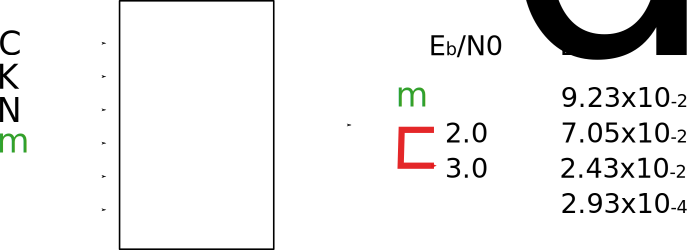
\includegraphics{simu/in_out/in_out}
  \caption{Input simulation parameters and output BER results.}
  \label{fig:intro_in_out}
\end{figure}

\begin{figure}[htp]
  \centering
  \subfloat[][Polar codes.]        {\includegraphics[width=0.30\textwidth]{simu/bfer/bfer_polar} \label{fig:intro_bfer_polar}}  \quad{}
  \subfloat[][LDPC codes.]         {\includegraphics[width=0.30\textwidth]{simu/bfer/bfer_ldpc}  \label{fig:intro_bfer_ldpc}}   \quad{}
  \subfloat[][Turbo codes.]        {\includegraphics[width=0.30\textwidth]{simu/bfer/bfer_turbo} \label{fig:intro_bfer_turbo}}  \\
  \subfloat[][Turbo product codes.]{\includegraphics[width=0.30\textwidth]{simu/bfer/bfer_tpc}   \label{fig:intro_bfer_tpc}}    \quad{}
  \subfloat[][BCH \& RS codes.]    {\includegraphics[width=0.30\textwidth]{simu/bfer/bfer_bch_rs}\label{fig:intro_bfer_bch_rs}} \quad{}
  \subfloat[][Convolutional codes.]{\includegraphics[width=0.30\textwidth]{simu/bfer/bfer_rsc}   \label{fig:intro_bfer_rsc}}
  \caption{\AFFECT simulation of various code families.}
  \label{fig:intro_bfer}
\end{figure}

On the eve of the 5G mobile communication generation, the challenge is now to
design communication systems able to transmit huge amounts of data in a short
time, at a small energy cost, in a wide variety of environments. Researchers
work at refining existing coding schemes further, to get low residual error
rates with fast, flexible, low complexity decoders.

The validation of a coding scheme requires estimating its error rate
performance. Usually, no simple mathematical model exists to predict such
performance. The only practical solution is to perform a Monte Carlo simulation
of the whole chain: some data are randomly generated, encoded, modulated,
noised, decoded, and the performance is then estimated by measuring the Bit
Error Rate (BER) and the Frame Error Rate (FER) at the sink. This process leads
to three main problems:

\begin{enumerate}
  \item \textbf{Simulation time:}
    100 erroneous frames must be simulated to accurately estimate the FER/BER.
    Thus, measuring a FER of $10^{-7}$ requires simulating the transmission of
    $\sim100\times 10^7=10^9$ frames. Assuming a frame of 1000~bits, the
    simulator must then emulate the transmission of $10^{12}$~bits. Keeping in
    mind that the decoding algorithm complexity may be significant, several
    weeks or months may be required to accurately estimate the FER/BER of a
    coding scheme.

  \item \textbf{Algorithmic heterogeneity:} A large number of channel codes have
    been designed over time. For each kind of code, several decoding algorithms
    are available. While it is straightforward to describe a unique coding
    scheme, it is more challenging to have a unified software description that
    supports all the coding schemes and their associated algorithms. This
    difficulty comes from the heterogeneity of the data structure necessary to
    describe a channel code and the associated decoder: turbo codes use
    trellises, LDPC codes are well-defined on factor graphs and polar codes are
    efficiently decoded using binary trees.

  \item \textbf{Reproducibility:} It is usually tedious to reproduce results
    from the literature. This can be explained by the large amount of empirical
    parameters necessary to define one communication system, and the fact that
    not all of them are always reported in publications. Moreover, the simulator
    source codes are rarely publicly available. Consequently, a large amount of
    time is spent ``reinventing the wheel'' just to be able to compare to the
    state-of-the-art results.
\end{enumerate}

The long simulation times make it desirable to have \textbf{high throughput
implementations}. The algorithmic heterogeneity requires \textbf{flexible,
modular software}. The reproducibility issue pushes towards a \textbf{portable}
and \textbf{open-source software}. These are the purposes of \AFFECT.

\section{Base Station and Cloud-RAN}

\begin{itemize}
  \item besoin d'implémentations software pour gagner en flexibilité et réduire
    les coûts par rapport au hardware dans les stations de base par ex. (SDR)
\end{itemize}

\section{Software Defined Radio (SDR)}

\section{Objectives}

\begin{itemize}
  \item High Performance
  \item Portability
  \item Algorithmic Heterogeneity
  \item Code re-use, pour éviter de tout jeter à chaque nouvel algo
\end{itemize}
